\section{Game engine architecture}
The game engine forms an environment for the agent by keeping track of the game state
(including scores), providing the available actions (moves), and generating possible
future states and their probabilities in the game tree based on the current knowledge.
The number of possible states in Carcassonne quickly rises as more tiles are placed on
the board leading to its high branching factor ($b = 55$ on average \cite{MasterThesisCarcassonne}).
To maximize the number of states that can be included in the search tree,
the team opted to implement the game engine from scratch using a fast compilable
language to later bridge it with an agent implemented in a language
that is better suited for developing AI applications.

Originally, the engine was supposed to be extended to support some game expansions
but eventually, this work had to be dropped due to slower-than-anticipated progress on
the core aspects of the project.

This section will focus on the architecture of this engine and how the communication within the whole system works.

\subsection{Overview of architecture}
% Opisanie architektury silnika, sposobu komunikacji między komponentami, a także za co one odpowiadają.

In this section, the project of game architecture will be discussed.
Figure \ref{fig:SystemArchitecture} shows a diagram of the whole system as implemented by the team.
Computations related to processing games are performed on a CPU,
while agents should be trained on a GPU.

\begin{figure*}
	\centering
	\scalebox{.48}{% Generated with:
% $ java -jar plantuml.jar -tlatex:nopreamble arch.pu
% generated by Plantuml 1.2024.8
\definecolor{plantucolor0000}{RGB}{24,24,24}
\definecolor{plantucolor0001}{RGB}{0,0,0}
\definecolor{plantucolor0002}{RGB}{241,241,241}
\begin{tikzpicture}[yscale=-1
,pstyle0/.style={color=plantucolor0000,line width=1.0pt}
,pstyle1/.style={color=black,line width=1.5pt}
,pstyle2/.style={color=plantucolor0000,fill=plantucolor0002,line width=0.5pt}
,pstyle3/.style={color=plantucolor0000,line width=0.5pt}
,pstyle5/.style={color=plantucolor0000,fill=plantucolor0000,line width=1.0pt}
,pstyle6/.style={color=plantucolor0000,line width=4.0pt}
,pstyle7/.style={color=plantucolor0000,fill=plantucolor0000,line width=4.0pt}
]
\draw[pstyle0] (38pt,97pt) -- (48pt,87pt) -- (517pt,87pt) -- (517pt,352pt) -- (507pt,362pt) -- (38pt,362pt) -- (38pt,97pt) -- cycle;
\draw[pstyle0] (507pt,97pt) -- (517pt,87pt);
\draw[pstyle0] (38pt,97pt) -- (507pt,97pt);
\draw[pstyle0] (507pt,97pt) -- (507pt,362pt);
\node at (260.99pt,100pt)[below right,color=black,inner sep=0]{\textbf{CPU}};
\draw[pstyle1] (196.5pt,129pt) -- (261.53pt,129pt) arc(270:360:3.75pt)  -- (271.03pt,145pt) -- (456.5pt,145pt) arc(270:360:2.5pt)  -- (459pt,335.5pt) arc(0:90:2.5pt)  -- (196.5pt,338pt) arc(90:180:2.5pt)  -- (194pt,131.5pt) arc(180:270:2.5pt) ;
\draw[pstyle1] (194pt,145pt) -- (271.03pt,145pt);
\node at (198pt,131pt)[below right,color=black,inner sep=0]{\textbf{GameEngine}};
\draw[pstyle0] (16pt,416pt) -- (26pt,406pt) -- (158pt,406pt) -- (158pt,486pt) -- (148pt,496pt) -- (16pt,496pt) -- (16pt,416pt) -- cycle;
\draw[pstyle0] (148pt,416pt) -- (158pt,406pt);
\draw[pstyle0] (16pt,416pt) -- (148pt,416pt);
\draw[pstyle0] (148pt,416pt) -- (148pt,496pt);
\node at (70.125pt,419pt)[below right,color=black,inner sep=0]{\textbf{GPU}};
\draw[pstyle2] (94.5pt,148pt) arc (180:270:5pt) -- (99.5pt,143pt) -- (172.14pt,143pt) arc (270:360:5pt) -- (177.14pt,148pt) -- (177.14pt,178pt) arc (0:90:5pt) -- (172.14pt,183pt) -- (99.5pt,183pt) arc (90:180:5pt) -- (94.5pt,178pt) -- cycle;
\draw[pstyle2] (157.14pt,148pt) rectangle (172.14pt,158pt);
\draw[pstyle2] (155.14pt,150pt) rectangle (159.14pt,152pt);
\draw[pstyle2] (155.14pt,154pt) rectangle (159.14pt,156pt);
\node at (109.5pt,163pt)[below right,color=black,inner sep=0]{Visualiser};
\draw[pstyle2] (54.5pt,284pt) arc (180:270:5pt) -- (59.5pt,279pt) -- (172.73pt,279pt) arc (270:360:5pt) -- (177.73pt,284pt) -- (177.73pt,314pt) arc (0:90:5pt) -- (172.73pt,319pt) -- (59.5pt,319pt) arc (90:180:5pt) -- (54.5pt,314pt) -- cycle;
\draw[pstyle2] (157.73pt,284pt) rectangle (172.73pt,294pt);
\draw[pstyle2] (155.73pt,286pt) rectangle (159.73pt,288pt);
\draw[pstyle2] (155.73pt,290pt) rectangle (159.73pt,292pt);
\node at (69.5pt,299pt)[below right,color=black,inner sep=0]{TrainingSupervisor};
\draw[pstyle2] (338.5pt,153pt) -- (401.02pt,153pt) ..controls (406.02pt,153pt) and (406.02pt,163pt) .. (406.02pt,163pt) ..controls (406.02pt,163pt) and (406.02pt,173pt) .. (401.02pt,173pt) -- (338.5pt,173pt) ..controls (333.5pt,173pt) and (333.5pt,163pt) .. (333.5pt,163pt) ..controls (333.5pt,163pt) and (333.5pt,153pt) .. (338.5pt,153pt);
\draw[pstyle3] (401.02pt,153pt) ..controls (396.02pt,153pt) and (396.02pt,163pt) .. (396.02pt,163pt) ..controls (396.02pt,173pt) and (401.02pt,173pt) .. (401.02pt,173pt);
\node at (338.5pt,158pt)[below right,color=black,inner sep=0]{BatchBuffer};
\draw[pstyle2] (253.5pt,289pt) arc (180:270:5pt) -- (258.5pt,284pt) -- (305.23pt,284pt) arc (270:360:5pt) -- (310.23pt,289pt) -- (310.23pt,309pt) arc (0:90:5pt) -- (305.23pt,314pt) -- (258.5pt,314pt) arc (90:180:5pt) -- (253.5pt,309pt) -- cycle;
\node at (263.5pt,294pt)[below right,color=black,inner sep=0]{Worker1};
\draw[pstyle2] (345.5pt,289pt) arc (180:270:5pt) -- (350.5pt,284pt) -- (397.23pt,284pt) arc (270:360:5pt) -- (402.23pt,289pt) -- (402.23pt,309pt) arc (0:90:5pt) -- (397.23pt,314pt) -- (350.5pt,314pt) arc (90:180:5pt) -- (345.5pt,309pt) -- cycle;
\node at (355.5pt,294pt)[below right,color=black,inner sep=0]{Worker2};
\node at (428.075pt,203pt)[below right,color=black,inner sep=0]{LoggerOutput};
\draw[color=plantucolor0000,fill=plantucolor0002,line width=1.5pt] (453pt,225pt) rectangle (465pt,237pt);
\draw[pstyle2] (32.5pt,445pt) arc (180:270:5pt) -- (37.5pt,440pt) -- (136.7pt,440pt) arc (270:360:5pt) -- (141.7pt,445pt) -- (141.7pt,475pt) arc (0:90:5pt) -- (136.7pt,480pt) -- (37.5pt,480pt) arc (90:180:5pt) -- (32.5pt,475pt) -- cycle;
\draw[pstyle2] (121.7pt,445pt) rectangle (136.7pt,455pt);
\draw[pstyle2] (119.7pt,447pt) rectangle (123.7pt,449pt);
\draw[pstyle2] (119.7pt,451pt) rectangle (123.7pt,453pt);
\node at (47.5pt,460pt)[below right,color=black,inner sep=0]{Pytorch/CUDA};
\draw[pstyle2] (263.5pt,12pt) arc (180:270:5pt) -- (268.5pt,7pt) -- (327.52pt,7pt) arc (270:360:5pt) -- (332.52pt,12pt) -- (332.52pt,35pt) arc (0:90:5pt) -- (327.52pt,40pt) -- (268.5pt,40pt) arc (90:180:5pt) -- (263.5pt,35pt) -- cycle;
\draw[pstyle2] (315.52pt,12pt) -- (315.52pt,26pt) -- (327.52pt,26pt) -- (327.52pt,18pt) -- (321.52pt,12pt) -- (315.52pt,12pt) -- cycle;
\draw[pstyle3] (321.52pt,12pt) -- (321.52pt,18pt);
\draw[pstyle3] (327.52pt,18pt) -- (321.52pt,18pt);
\node at (273.5pt,20pt)[below right,color=black,inner sep=0]{gameLog};
\draw[pstyle0] (363.95pt,173.21pt) ..controls (348.88pt,196.15pt) and (312.8842pt,250.9752pt) .. (294.7342pt,278.6052pt);
\draw[pstyle5] (291.44pt,283.62pt) -- (299.7245pt,278.2939pt) -- (294.1852pt,279.441pt) -- (293.0381pt,273.9017pt) -- (291.44pt,283.62pt) -- cycle;
\draw[pstyle0] (370.27pt,173.21pt) ..controls (370.96pt,196.15pt) and (372.572pt,249.9926pt) .. (373.392pt,277.6226pt);
\draw[pstyle5] (373.57pt,283.62pt) -- (377.3013pt,274.5053pt) -- (373.4217pt,278.6222pt) -- (369.3048pt,274.7426pt) -- (373.57pt,283.62pt) -- cycle;
\draw[pstyle0] (338.3696pt,32.1399pt) ..controls (366.7796pt,39.0599pt) and (400.13pt,51.68pt) .. (423pt,79pt) ..controls (461.23pt,124.67pt) and (460.28pt,204.02pt) .. (459.31pt,224.87pt);
\draw[pstyle5] (332.54pt,30.72pt) -- (340.3377pt,36.7363pt) -- (337.398pt,31.9033pt) -- (342.231pt,28.9635pt) -- (332.54pt,30.72pt) -- cycle;
\draw[pstyle0] (263.53pt,40.02pt) ..controls (244.27pt,49.64pt) and (220.5pt,63.18pt) .. (202pt,79pt) ..controls (180.04pt,97.79pt) and (160.19pt,124.75pt) .. (148.12pt,142.79pt);
\draw[pstyle6] (188.2564pt,194.6698pt) ..controls (169.7577pt,203.2148pt) and (157.425pt,209.51pt) .. (154pt,213pt) ..controls (135.89pt,231.47pt) and (125.58pt,260.05pt) .. (120.39pt,278.9pt);
\draw[pstyle7] (193.7074pt,192.1624pt) -- (183.8594pt,192.2895pt) -- (189.1649pt,194.2519pt) -- (187.2025pt,199.5575pt) -- (193.7074pt,192.1624pt) -- cycle;
\node at (155pt,226pt)[below right,color=black,inner sep=0]{Action};
\draw[pstyle6] (193.7154pt,243.6133pt) ..controls (193.6039pt,243.7216pt) and (193.4923pt,243.8298pt) .. (193.3808pt,243.9378pt) ..controls (191.5955pt,245.6666pt) and (189.8006pt,247.3569pt) .. (188pt,249pt) ..controls (175.94pt,260.01pt) and (166.2778pt,267.1911pt) .. (153.3078pt,275.5811pt);
\draw[pstyle7] (148.27pt,278.84pt) -- (157.9993pt,277.3103pt) -- (152.4682pt,276.1243pt) -- (153.6542pt,270.5931pt) -- (148.27pt,278.84pt) -- cycle;
\node at (221pt,226pt)[below right,color=black,inner sep=0]{NewGameState};
\draw[pstyle6] (90.47pt,319.04pt) ..controls (73.75pt,333.2pt) and (53.33pt,354.14pt) .. (44pt,378pt) ..controls (35.36pt,400.09pt) and (47.2722pt,419.5087pt) .. (62.1422pt,435.5587pt);
\draw[pstyle7] (66.22pt,439.96pt) -- (63.0376pt,430.6395pt) -- (62.8219pt,436.2922pt) -- (57.1691pt,436.0765pt) -- (66.22pt,439.96pt) -- cycle;
\node at (45pt,379pt)[below right,color=black,inner sep=0]{NewGameState};
\draw[pstyle6] (119.1934pt,325.1575pt) ..controls (121.1134pt,343.5375pt) and (122pt,365.98pt) .. (117pt,390pt) ..controls (113.33pt,407.65pt) and (104.9pt,426.32pt) .. (97.91pt,439.78pt);
\draw[pstyle7] (118.57pt,319.19pt) -- (115.5267pt,328.5569pt) -- (119.0895pt,324.1629pt) -- (123.4834pt,327.7257pt) -- (118.57pt,319.19pt) -- cycle;
\node at (120pt,379pt)[below right,color=black,inner sep=0]{Action};
\end{tikzpicture}
}
	\caption{Diagram of the system's architecture}
	\label{fig:SystemArchitecture}
\end{figure*}

The GameEngine is responsible for evaluating requests it receives from the agents
ensuring that Carcassonne's rule set is followed. It maintains currently active games,
exposes the current state to the agents, generates possible moves for the given input,
and allows simulation of what game state a sequence of actions will lead to (before performing it
on an active game). Internally, GameEngine distributes the requests it receives among
multiple workers (lightweight threads) that can evaluate them simultaneously. Actions that
require state transitions are performed on a state's clone, while read-only operations
get performed on the original copy which is meant to enable efficient concurrency.

For each active game, GameEngine logs all of its states to that game's log file,
allowing for later consumption by Visualiser. Visualiser parses the logs
and presents the game in a graphical form, allowing for analysis by humans.

TrainingSupervisor is responsible for managing communication and supervising agents' training.
It should optimise communication by reducing data transfer between CPU and GPU.

The GameEngine (and Visualiser) is implemented in Go, while the agent and TrainingSupervisor
are implemented in Python. The use of Go for the engine was meant to allow for better performance of
the rule engine but it means that the TrainingSupervisor cannot communicate with it directly.
To solve this, the team used the gopy project \cite{gopy} to automatically generate
Python bindings \cite{LanguageBindings} for the Go package. This leads to a larger overhead than
using manually-written CPython extension would but this has been considered acceptable as most of
the CPU-bound work happens in the GameEngine itself, not at the communication layer.

\subsection{Components of a solution}
% Opisanie elementów z jakich się składa rozgrywka m.in.: kafelki i ich elementy, gracze, a także uwzględnione rozszerzenia gry Carcassonne.

The game Carcassone is played by placing tiles \cite{CarcassoneRules}. Each tile is represented by a set of features on it. All features are defined by their type, such as road, city, field or monastery, a modifier that modifies the calculation process, and the sides which indicate on which edges the feature is present. In this project, there is only one modifier used - the shield. The engine was designed to accommodate game extensions.

A feature's side is a byte-sized value, in which each bit defines whether the feature is present on a specific half of the tile's edge as shown on Figure \ref{fig:SIDES}. Features such as roads, are represented by a whole edge formed by combining two sides e.g., the TopLeft and TopRight sides.
\begin{figure}
    \centering
    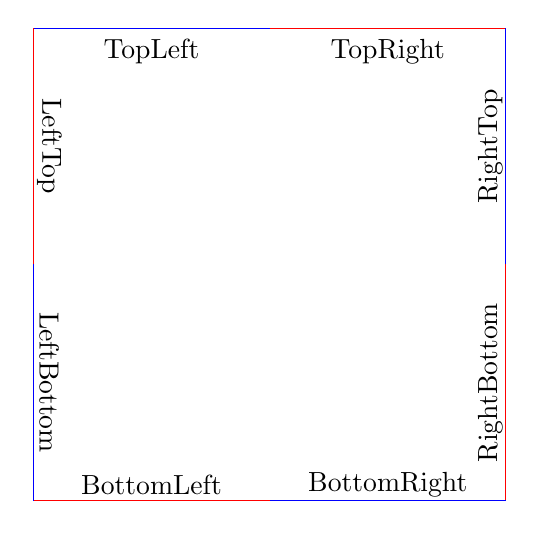
\begin{tikzpicture}
        %top line
        \draw [blue] (-3,3) -- (0,3);
        \draw [red] (0,3) -- (3,3);
        %right line
        \draw [blue] (3,3) -- (3,0);
        \draw [red] (3,0) -- (3,-3);
        %bottom line
        \draw [blue] (3,-3) -- (0,-3);
        \draw [red] (0,-3) -- (-3,-3);
        %left line
        \draw [blue] (-3,-3) -- (-3,0);
        \draw [red] (-3,0) -- (-3,3);
        
        \node at (-1.5, 2.7) {TopLeft};
        \node at (1.5, 2.7) {TopRight};
        
        \node [rotate=90] at (2.8, 1.5) {RightTop};
        \node [rotate=90] at (2.8, -1.5) {RightBottom};
        
        \node at (-1.5, -2.8) {BottomLeft};
        \node at (1.5, -2.8) {BottomRight};
        
	% czy może obrót 90stopni?
        \node [rotate=270] at (-2.8, 1.5) {LeftTop};
        \node [rotate=270] at (-2.8, -1.5) {LeftBottom};
    \end{tikzpicture}
    \caption{Side representation} \label{fig:SIDES}
\end{figure}

The tiles described do not contain information about their position or meeple placement. This information is located in the PlacedTile struct. The board is represented as a tile set containing tiles used in the game, for verification whether the tile a player wants to place is legal. Moreover, it contains a slice of placed tiles in the same order as the tile set. Additionally, the board includes a city manager used for merging cities, scoring and checking for legal meeple placements in the cities.

A single game is represented by a board, a shuffled deck of tiles, and players partaking in it. Each player knows their score and the number of meeples of each type available to them.

Our solution has been designed to be modifiable by adding extensions to the game. Generalizations, such as meeple type or feature type, allow for the easy implementation of new potential features, e.g. rivers.

\subsection{Game flow}
% Opisanie wykonywanych akcji podejmowanych przez silnik gry: wylosowanie kafelka ze stosu, wyliczenie legalnych ułożeń kafelka, wybór położenia i wyliczanie punktacji za jego położenie.

This section will present the whole flow of the game and the way it was implemented in the engine.
Figure \ref{fig:GameFlow} shows a state diagram of the game.

\begin{figure*}
	\centering
	\scalebox{.42}{% Generated with:
% $ java -jar plantuml.jar -tlatex:nopreamble state-diagram.pu
% generated by Plantuml 1.2024.8       
\definecolor{plantucolor0000}{RGB}{241,241,241}
\definecolor{plantucolor0001}{RGB}{24,24,24}
\definecolor{plantucolor0002}{RGB}{0,0,0}
\definecolor{plantucolor0003}{RGB}{34,34,34}
\begin{tikzpicture}[yscale=-1
,pstyle0/.style={color=plantucolor0001,fill=plantucolor0000,line width=0.5pt}
,pstyle1/.style={color=plantucolor0003,fill=plantucolor0003,line width=1.0pt}
,pstyle3/.style={color=plantucolor0001,line width=1.0pt}
,pstyle4/.style={color=plantucolor0001,fill=plantucolor0001,line width=1.0pt}
]
\draw[pstyle0] (159.5pt,565pt) arc (180:270:20pt) -- (179.5pt,545pt) -- (240.07pt,545pt) arc (270:360:20pt) -- (260.07pt,565pt) -- (260.07pt,565pt) arc (0:90:20pt) -- (240.07pt,585pt) -- (179.5pt,585pt) arc (90:180:20pt) -- (159.5pt,565pt) -- cycle;
\node at (164.5pt,560pt)[below right,color=black,inner sep=0]{Active player change};
\draw[pstyle0] (353.5pt,139pt) arc (180:270:20pt) -- (373.5pt,119pt) -- (404.08pt,119pt) arc (270:360:20pt) -- (424.08pt,139pt) -- (424.08pt,139pt) arc (0:90:20pt) -- (404.08pt,159pt) -- (373.5pt,159pt) arc (90:180:20pt) -- (353.5pt,139pt) -- cycle;
\node at (358.5pt,134pt)[below right,color=black,inner sep=0]{1A. Tile draw};
\draw[pstyle0] (233pt,127pt) -- (245pt,139pt) -- (233pt,151pt) -- (221pt,139pt) -- (233pt,127pt) -- cycle;
\draw[pstyle0] (311pt,27pt) arc (180:270:20pt) -- (331pt,7pt) -- (372.8pt,7pt) arc (270:360:20pt) -- (392.8pt,27pt) -- (392.8pt,27pt) arc (0:90:20pt) -- (372.8pt,47pt) -- (331pt,47pt) arc (90:180:20pt) -- (311pt,27pt) -- cycle;
\node at (316pt,22pt)[below right,color=black,inner sep=0]{Tile is discarded};
\draw[pstyle0] (472pt,127pt) -- (484pt,139pt) -- (472pt,151pt) -- (460pt,139pt) -- (472pt,127pt) -- cycle;
\draw[pstyle0] (464.5pt,251pt) arc (180:270:20pt) -- (484.5pt,231pt) -- (537.4pt,231pt) arc (270:360:20pt) -- (557.4pt,251pt) -- (557.4pt,251pt) arc (0:90:20pt) -- (537.4pt,271pt) -- (484.5pt,271pt) arc (90:180:20pt) -- (464.5pt,251pt) -- cycle;
\node at (469.5pt,246pt)[below right,color=black,inner sep=0]{1B. Tile placement};
\draw[pstyle0] (282pt,239pt) -- (294pt,251pt) -- (282pt,263pt) -- (270pt,251pt) -- (282pt,239pt) -- cycle;
\draw[pstyle0] (417pt,239pt) -- (429pt,251pt) -- (417pt,263pt) -- (405pt,251pt) -- (417pt,239pt) -- cycle;
\draw[pstyle0] (500pt,363pt) arc (180:270:20pt) -- (520pt,343pt) -- (577.94pt,343pt) arc (270:360:20pt) -- (597.94pt,363pt) -- (597.94pt,363pt) arc (0:90:20pt) -- (577.94pt,383pt) -- (520pt,383pt) arc (90:180:20pt) -- (500pt,363pt) -- cycle;
\node at (505pt,358pt)[below right,color=black,inner sep=0]{2. Figure placement};
\draw[pstyle0] (310.5pt,464pt) arc (180:270:20pt) -- (330.5pt,444pt) -- (379.64pt,444pt) arc (270:360:20pt) -- (399.64pt,464pt) -- (399.64pt,464pt) arc (0:90:20pt) -- (379.64pt,484pt) -- (330.5pt,484pt) arc (90:180:20pt) -- (310.5pt,464pt) -- cycle;
\node at (315.5pt,459pt)[below right,color=black,inner sep=0]{3. Feature scoring};
\draw[pstyle0] (63.5pt,139pt) arc (180:270:20pt) -- (83.5pt,119pt) -- (110.12pt,119pt) arc (270:360:20pt) -- (130.12pt,139pt) -- (130.12pt,139pt) arc (0:90:20pt) -- (110.12pt,159pt) -- (83.5pt,159pt) arc (90:180:20pt) -- (63.5pt,139pt) -- cycle;
\node at (68.5pt,134pt)[below right,color=black,inner sep=0]{Final scoring};
\draw[pstyle1] (93pt,464pt) ellipse (10pt and 10pt);
\draw[pstyle0] (62pt,565pt) arc (180:270:20pt) -- (82pt,545pt) -- (103.88pt,545pt) arc (270:360:20pt) -- (123.88pt,565pt) -- (123.88pt,565pt) arc (0:90:20pt) -- (103.88pt,585pt) -- (82pt,585pt) arc (90:180:20pt) -- (62pt,565pt) -- cycle;
\node at (67pt,560pt)[below right,color=black,inner sep=0]{Preparation};
\draw[color=plantucolor0003,line width=1.0pt] (17pt,139pt) ellipse (11pt and 11pt);
\draw[pstyle1] (17pt,139pt) ellipse (6pt and 6pt);
\draw[pstyle3] (93pt,474.14pt) ..controls (93pt,490.12pt) and (93pt,517.49pt) .. (93pt,538.77pt);
\draw[pstyle4] (93pt,544.77pt) -- (97pt,535.77pt) -- (93pt,539.77pt) -- (89pt,535.77pt) -- (93pt,544.77pt) -- cycle;
\draw[pstyle3] (124.08pt,565pt) ..controls (135.83pt,565pt) and (141.57pt,565pt) .. (153.32pt,565pt);
\draw[pstyle4] (159.32pt,565pt) -- (150.32pt,561pt) -- (154.32pt,565pt) -- (150.32pt,569pt) -- (159.32pt,565pt) -- cycle;
\draw[pstyle3] (202.54pt,544.98pt) ..controls (195.49pt,525.29pt) and (186pt,493.47pt) .. (186pt,465pt) ..controls (186pt,250pt) and (186pt,250pt) .. (186pt,250pt) ..controls (186pt,207.63pt) and (212.2854pt,167.7663pt) .. (224.4054pt,151.3563pt);
\draw[pstyle4] (227.97pt,146.53pt) -- (219.4055pt,151.3931pt) -- (224.9995pt,150.552pt) -- (225.8406pt,156.1459pt) -- (227.97pt,146.53pt) -- cycle;
\draw[pstyle3] (245.24pt,139pt) ..controls (268.23pt,139pt) and (312.64pt,139pt) .. (347.21pt,139pt);
\draw[pstyle4] (353.21pt,139pt) -- (344.21pt,135pt) -- (348.21pt,139pt) -- (344.21pt,143pt) -- (353.21pt,139pt) -- cycle;
\node at (263.25pt,125pt)[below right,color=black,inner sep=0]{Stack not empty};
\draw[pstyle3] (136.62pt,139pt) ..controls (165.88pt,139pt) and (200.67pt,139pt) .. (220.78pt,139pt);
\draw[pstyle4] (130.62pt,139pt) -- (139.62pt,143pt) -- (135.62pt,139pt) -- (139.62pt,135pt) -- (130.62pt,139pt) -- cycle;
\node at (148.75pt,125pt)[below right,color=black,inner sep=0]{Stack empty};
\draw[pstyle3] (424.66pt,139pt) ..controls (436.37pt,139pt) and (442.09pt,139pt) .. (453.8pt,139pt);
\draw[pstyle4] (459.8pt,139pt) -- (450.8pt,135pt) -- (454.8pt,139pt) -- (450.8pt,143pt) -- (459.8pt,139pt) -- cycle;
\draw[pstyle3] (377.3231pt,51.2142pt) ..controls (405.2631pt,76.8242pt) and (448.8pt,116.73pt) .. (465.8pt,132.32pt);
\draw[pstyle4] (372.9pt,47.16pt) -- (376.8318pt,56.19pt) -- (376.5859pt,50.5385pt) -- (382.2374pt,50.2926pt) -- (372.9pt,47.16pt) -- cycle;
\node at (416pt,78pt)[below right,color=black,inner sep=0]{no valid placement};
\draw[pstyle3] (331.27pt,47.16pt) ..controls (303.57pt,72.77pt) and (260.4153pt,112.6565pt) .. (243.5553pt,128.2465pt);
\draw[pstyle4] (239.15pt,132.32pt) -- (248.4736pt,129.1467pt) -- (242.8211pt,128.9254pt) -- (243.0423pt,123.2729pt) -- (239.15pt,132.32pt) -- cycle;
\draw[pstyle3] (474.93pt,148.27pt) ..controls (481.1pt,165.66pt) and (493.5342pt,200.7452pt) .. (502.1642pt,225.0752pt);
\draw[pstyle4] (504.17pt,230.73pt) -- (504.9312pt,220.9106pt) -- (502.4985pt,226.0177pt) -- (497.3914pt,223.585pt) -- (504.17pt,230.73pt) -- cycle;
\node at (493pt,190pt)[below right,color=black,inner sep=0]{has valid placement};
\draw[pstyle3] (489.44pt,230.75pt) ..controls (474.04pt,217.75pt) and (452.13pt,202.02pt) .. (429.5pt,195pt) ..controls (373.78pt,177.7pt) and (313.2289pt,224.0591pt) .. (292.9289pt,241.4291pt);
\draw[pstyle4] (288.37pt,245.33pt) -- (297.8089pt,242.518pt) -- (292.1691pt,242.0793pt) -- (292.6077pt,236.4395pt) -- (288.37pt,245.33pt) -- cycle;
\draw[pstyle3] (280.53pt,261.64pt) ..controls (277.54pt,283.91pt) and (272.38pt,340.35pt) .. (289pt,383pt) ..controls (298.28pt,406.82pt) and (313.2619pt,424.6538pt) .. (328.6119pt,439.5338pt);
\draw[pstyle4] (332.92pt,443.71pt) -- (329.242pt,434.5737pt) -- (329.3299pt,440.2299pt) -- (323.6738pt,440.3178pt) -- (332.92pt,443.71pt) -- cycle;
\node at (290pt,358pt)[below right,color=black,inner sep=0]{figure count == 0};
\draw[pstyle3] (294.46pt,251pt) ..controls (320.31pt,251pt) and (373.48pt,251pt) .. (398.96pt,251pt);
\draw[pstyle4] (404.96pt,251pt) -- (395.96pt,247pt) -- (399.96pt,251pt) -- (395.96pt,255pt) -- (404.96pt,251pt) -- cycle;
\node at (312.5pt,237pt)[below right,color=black,inner sep=0]{figure count != 0};
\draw[pstyle3] (414.49pt,260.53pt) ..controls (405.34pt,291.68pt) and (375.2818pt,393.9735pt) .. (362.2918pt,438.1735pt);
\draw[pstyle4] (360.6pt,443.93pt) -- (366.9754pt,436.423pt) -- (362.0098pt,439.1329pt) -- (359.3pt,434.1673pt) -- (360.6pt,443.93pt) -- cycle;
\node at (391pt,358pt)[below right,color=black,inner sep=0]{no figure};
\draw[pstyle3] (423.01pt,257.01pt) ..controls (440.97pt,271.97pt) and (490.2504pt,313.0492pt) .. (521.4304pt,339.0292pt);
\draw[pstyle4] (526.04pt,342.87pt) -- (521.6862pt,334.0357pt) -- (522.1987pt,339.6693pt) -- (516.5651pt,340.1818pt) -- (526.04pt,342.87pt) -- cycle;
\node at (487pt,302pt)[below right,color=black,inner sep=0]{has figure};
\draw[pstyle3] (511.59pt,383.09pt) ..controls (477.24pt,400.62pt) and (431.9546pt,423.7332pt) .. (397.6346pt,441.2432pt);
\draw[pstyle4] (392.29pt,443.97pt) -- (402.1247pt,443.4429pt) -- (396.7438pt,441.6977pt) -- (398.489pt,436.3167pt) -- (392.29pt,443.97pt) -- cycle;
\draw[pstyle3] (327.04pt,484.09pt) ..controls (301.37pt,501.62pt) and (268.4754pt,524.0772pt) .. (242.8254pt,541.5872pt);
\draw[pstyle4] (237.87pt,544.97pt) -- (247.5584pt,543.1994pt) -- (241.9995pt,542.151pt) -- (243.0479pt,536.5921pt) -- (237.87pt,544.97pt) -- cycle;
\draw[pstyle3] (34.25pt,139pt) ..controls (45.98pt,139pt) and (51.7pt,139pt) .. (63.43pt,139pt);
\draw[pstyle4] (28.25pt,139pt) -- (37.25pt,143pt) -- (33.25pt,139pt) -- (37.25pt,135pt) -- (28.25pt,139pt) -- cycle;
\end{tikzpicture}
}
	\caption{Carcassonne's state diagram}
	\label{fig:GameFlow}
\end{figure*}

Before the game can start, a few actions need to be performed as part of the \textbf{Preparation} stage:
\begin{itemize}
	\item putting a start tile on the board,
	\item generating a stack of all (remaining) tiles in random order,
	\item setting the figure count for each player to $7$,
	\item resetting the scores of all players to $0$,
	\item choosing the player order.
\end{itemize}
In the implementation, these steps are executed when a new game object (along with its board
and players) is created. The player order is fixed and the stack is internal to the engine
to avoid leaking its order to the agents.

Once the game starts, the players take turns with the drawn tiles. The engine takes tiles from
the top of game's stack of remaining tiles (\textbf{Tile draw}) until it finds one that can be
placed somewhere on the board which it then includes as part of the state passed to the agent.
When no tiles are left on the stack, the engine proceeds to the \textbf{Final scoring} stage
(described later).

Once the agent knows the tile it needs to place, it needs to choose \textbf{Tile placement} and,
if it has any figures, \textbf{Figure placement}. In the implementation, this is performed
as a single action - the agent has to choose both the position/rotation of the tile and the feature
to put a meeple on (if any) which it then sends as input to play the turn.
The engine allows the agent to ask for valid tile placements as well as valid features to
place meeple on for the given tile, taking into account whether that feature (which can spread
over several tiles) does not already have a meeple placed. When a meeple is placed,
the player's meeple count is decremented by $1$.

After the tile is placed (following the validation of the move by the engine),
we need to proceed with \textbf{Feature scoring}. During this stage, all features that have been
completed after the tile was placed have to be identified, the control over them needs to be resolved,
and then points need to be awarded to the controlling players and their meeple counts updated.
The implementation performs this when handling the request of placing a tile (with meeple) on the board.

After \textbf{Feature scoring}, the next player takes a turn and the game continues
until the stack of remaining tiles is empty. To get the final results,
\textbf{Final scoring} is performed after emptying the stack. This consists of scoring
all uncompleted features and all features known as end-of-game features
(in the base game, just fields).

\subsection{Communication within a system} \label{communication}
% Opisanie komunikacji pomiędzy silnikiem gry, a sieciami neuronowymi uczonymi na karcie graficznej. Aktualizacja stanu gry w zależności od akcji podejmowanych przez agenta.

The game engine is capable of handling multiple game instances, by using Go pipelines and goroutines \cite{GolangPipeline}, which allows for many agents to play and learn simultaneously. The engine provides several request types necessary for the agents, to retrieve information about the game. There are five such requests:
\begin{itemize}
    \item CloneGame - used for creating a separate clone of a game. It allows the agent to expand the game tree, and each clone can be modified by the agent, by simulating its next potential move.
    \item GetRemainingTiles - returns all available tiles that have not yet been placed. With this data, the agent can expand the game tree for each possible move that might occur. The returned tiles come with information about their probability.
    \item GetLegalMoves - returns all legal moves for a given tile. It considers where the tile can be placed and where are the possible meeple placements on it.
    \item GetMidGameScore - returns the information about the score for all players, calculated as if the game has just finished.
    \item PlayTurn - allows the agent to play a turn using a given tile, and modifies the game state. It returns the new state of the game.
\end{itemize}

With these requests, the agent is capable of building its game tree and performing the selected actions.

To provide the neural network with the game state, a serialization process is required. The serialized game contains all players' statistics (meeple counts, score) and all tiles on the board. The placed tiles on the board are represented in the binary format to ensure a fixed memory size of 8 bytes. The slice of binary tiles consists of all tiles in the same order as tiles in tile set. The tiles in this array that are not yet placed are set to zero.

\subsection{Performance}

Once the engine implementation reached a certain stage,
the team created a benchmark suite measuring the performance of the engine’s operations.
This allowed us to assess if the overall performance was acceptable and ensured that
no performance regressions were introduced at a later stage of the implementation.

The benchmark suite consists of two types of benchmark tests.
The first one is feature tests and the second one is engine request tests.


\subsubsection{Feature tests}

The aim of the feature tests is measuring the time that processing of
a specific feature type contributes to the overall time of turn processing.
During the measurement, a test for a specific feature places tiles consisting of
only that specific feature. For each feature, two testing strategies were used:
\begin{itemize}
	\item a test with a single game where each tile is placed on the right of the previous one,
          resulting in a long row of tiles consisting of that feature,
    \item a test with many shorter (in terms of the tile count) games,
          each ending with a short row of tiles consisting of that feature.
\end{itemize}

\subsubsection{Engine request tests}

The aim of the engine request tests is to measure the time of both the game processing
and the abstraction on top of it that the agents use. The time measured here reflects
how long the agent has to wait on requests to get responses. The individual tests measure
specific requests from the ones documented in the earlier section (\ref{communication}).

Each request is tested by simulating 100 semi-random games. In each turn, for each game instance,
the tested request is called and the total execution of the request is measured.
If the tested request mutates the game, it is evaluated on a temporary copy.

\subsubsection{Improving performance}

After evaluating the performance as well as testing the whole system with
an agent implementation, we've observed that the efficiency of the engine does not
realistically allow us to train an agent with a full standard tile set (72 tiles).
The expansion of a tree by just one level was already proving to be problematic.
To mitigate this, we worked on improving the engine's performance.

We found and implemented a few ideas for enhancing the efficiency of the system:
\begin{itemize}
	\item allowing to compare tile and placed tile types without needing to convert one to another,
    \item updating the null logger implementation to be a full no-op,
    \item allowing the engine to receive requests from the agent on multiple threads,
    \item changing the tile representation to simple integers of a constant size (i.e. no slices)
          that can be operated on with bitwise operations,
    \item holding just the shield count rather than the exact positions of shields in cities,
    \item decreasing the size of enum types such as feature type and shield flag to a single byte,
    \item decreasing the size of X and Y position coordinates to single-byte integers.
\end{itemize}
Some of the above solutions resulted in promising improvements,
while others offered smaller speedups or, in some cases, had the opposite effect.
Overall, the performance gains were not enough to allow for use in agent training.
